\chapter{TEMPLATE E STRATEGY}
Sono due pattern comportamentali.

\section{Template Method}
Definisce, in unico punto, lo scheletro di un algoritmo e delega alcuni passi, quelli che possono variare da oggetto ad oggetto, alle sottoclassi che avranno il compito 
di ridefinirli.

Prendiamo come esempio un framework che fornisce la classe Application e Document resposnsabili, rspettivamente, di aprire un documento e salvarlo e di rappresentare le
informazioni di un documento una volta in memoria.

Application, intesa come classe astratta, definirà l’algoritmo per aprire e leggere un documento in un metodo openDocument() che chiamerà al suo interno altri metodi 
di utilità, astratti, che saranno overridati dalle sottoclassi.

\medskip
\textbf{N.B.} Il template method non sono i metodi astratti ma è il metodo che li chiama che defnisce lo scheletro dell'algoritmo.

\begin{lstlisting}
public abstract class Application {
    private List<Document> docs;
    // costruttore...
    
    public final void openDocument(String path) {
        if (!canOpenDocument(path)) {
            // gestisce l'errore
        }

        Document doc = doCreateDocument(path);
        docs.add(doc);
        aboutToOpenDoc(doc);
        doc.open();
        doc.doRead();
    }

    protected abstract void aboutToOpenDoc(Document doc);
    protected abstract Document doCreateDocument(String path);
    protected abstract boolean canOpenDocument(String path);
}
\end{lstlisting}

Chi intenderà utilizzare il nostro framework dovrà estendere le classi Application e Document, ridefinendo i metodi astratti.


Il templateMethod porta all'\textit{hollywood principle}, ovvero sono le classi parent a chiamare i metodi delle sottoclassi e non l'inverso. 

\medskip
\textbf{N.B.} Sapendo che il templateMethod non cambiarà mai, allora potremmo renderlo final.

\subsection{Struttura e partecipanti}

\begin{figure}[H]
    \centering
    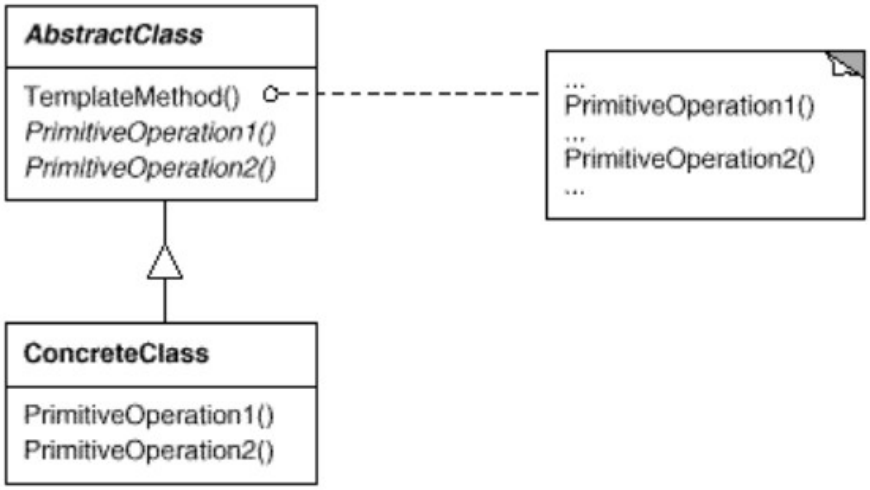
\includegraphics[width=0.4\linewidth]{../../immagini/templateMethod_Strategy/struttura_templateMethod}    
\end{figure}

\textbf{AbstractClass} 

\begin{itemize}
    \item \textit{definisce} le operazioni primitive astratte che rappresentano i passi di un algoritmo;
    \item \textit{Implementa} il template method che rappresenta l’algoritmo che, a sua volta, chiama le operazioni astratte.
\end{itemize}

\textbf{ConcreteClass} che implementa le operazioni primitive.

\section{Strategy}

Definisce una famiglia di algoritmi, incapsula ogni algoritmo e li rende intercambiabili, nascondo le informazioni interne dell’implementazione.

I Client devono essere consapevoli che esistono diverse strategie, avremo un overhead di comunicazione tra Context e Strategy e numero di oggetti nel sistema sarà 
maggiore.

Il pattern deve essere usato solo quando la \textit{variazione del comportamento} è fondamentale per i client.

Prendiamo ad esempio un Shop che può applicare più sconti, ad esempio quello percentuale, assoluto o nessuno sconto.

\begin{lstlisting}
public class Shop {

private DiscountStrategy discountStrategy;
    public Shop(DiscountStrategy discountStrategy) {
        this.discountStrategy = discountStrategy;
    }

    public void setDiscountStrategy(DiscountStrategy discountStrategy) {
        this.discountStrategy = discountStrategy
    }

    public int getTotal(int originalPrice) {
        return discountStrategy.applyDiscount(originalPrice);
    }
}
\end{lstlisting}

DiscountStrategy è la nostra interfaccia che mette a disposizione il metodo, astratto, applyDiscount(int) che sarà gestito in maniera differente in base alla tipologia
di sconto che vogliamo applicare.

\begin{multicols}{2}
    \begin{lstlisting}
        public interface DiscountStrategy {
            int applyDiscount(int originalPrice);
        }
    \end{lstlisting}
\columnbreak
    \begin{lstlisting}
        public class NoDiscountStrategy implements DiscountStrategy {
            @Override
            public int applyDiscount(int originalPrice) {
                return originalPrice;
            }
        }
    \end{lstlisting}
\end{multicols}

\begin{multicols}{2}
    \begin{lstlisting}
        public class AbsoluteDiscountStrategy implements DiscountStrategy {
        private int discount;
        
        public AbsoluteDiscountStrategy(int discount) {
            this.discount = discount;
        }

        @Override
        public int applyDiscount(int originalPrice) {
            return originalPrice - discount;
        }
    }    
    \end{lstlisting}
\columnbreak
    \begin{lstlisting}
        public class PercentageDiscountStrategy implements DiscountStrategy {
        private int percentage;
        
        public PercentageDiscountStrategy(int percentage) {
            this.percentage = percentage;
        }

        @Override
        public int applyDiscount(int originalPrice) {
            return originalPrice - (originalPrice * percentage / 100);
        }
    }
    \end{lstlisting}
\end{multicols}

\subsection{Struttura e partecipanti}

\begin{figure}[H]
    \centering   
    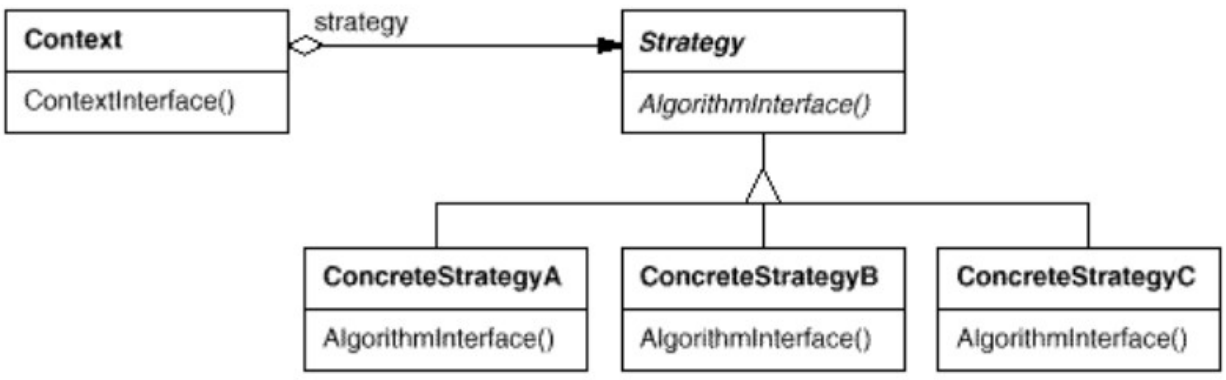
\includegraphics[width=0.5\linewidth]{../../immagini/templateMethod_Strategy/struttura_strategy}    
\end{figure}


\textbf{Strategy} dichiara l’interfaccia comune a tutti gli algoritmi supportati.

\textbf{ConcreteStrategy} implementa l’interfaccia Strategy e implementa l’algoritmo .

\textbf{Context} usa uno Strategy quando ha bisogno dell’algoritmo che, a runtime, sarà effettivamente implementato da un ConcreteStrategy.

\subsection{Differenza con il templateMethod}

Sembra simile al templateMethod, invece è completamente l'opposto.

Col templateMethod l'\textit{implementazione dell'algoritmo è fissa}, cambia solamente l'implementazione di alcuni suoi passi, mentre nello strategy è 
\textit{fisso il problema che intende risovere} l'algoritmo, il come deve essere risolto viene implementato dalle sottoclassi. 

Prendiamo come esempio l'ordinamento

\begin{itemize}
    \item con il templateMethod avremo il Bubblesort come algoritmo fisso, dove al suo interno potranno \textbf{cambiare alcuni suoi passi}, quindi le sottoclassi
    estenderanno la classe Bubblesort ed implementeranno i suoi passi astratti;
    \item con lo strartegy, si definisce un'interfaccia per l'ordinamento dove l'\textbf{algoritmo cambia}, a seconda del tipo di ordinamento,  
    (SelectionSort, InsertionSort, Bubblesort, ecc\dots..), quindi le sottoclasse implementeranno Ordinamento e ridefiniranno l'algoritmo a proprio piacimento.
\end{itemize}

Template Method sfrutta l’inheritance e l’overriding (meccanismo statico), mentre lo Strategy sfrutta l’object composition e delegation (meccanismo dinamico), 
infatti l’implementazione di strategy può essere anche modificata a runtime, ad esempio tramite il setter.